\chapter{Figures and Equations}\label{chap:method}

\section{Adding a figure}
Put figure files in the folder figures.
Figures are numbered by chapter, as in \figref{fig:sample}, and the caption goes below the figure.

\begin{figure}[htbp]
  \centering
  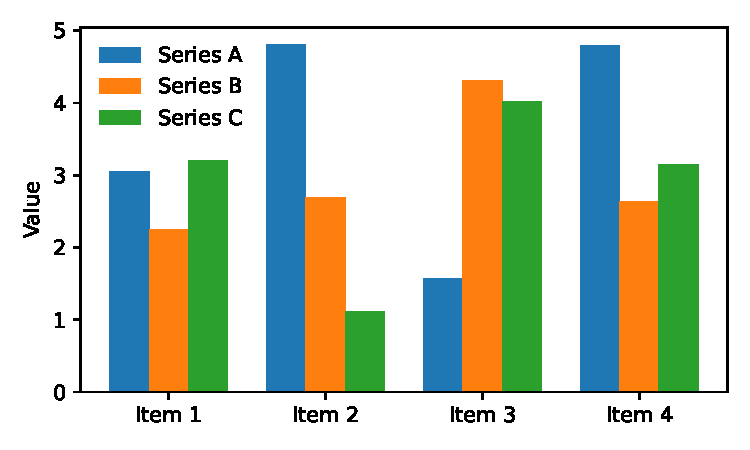
\includegraphics[width=0.7\linewidth]{figures/sample-chart.pdf}
  \caption{An example of a bar chart}\label{fig:sample}
  \source{by the author}
\end{figure}

\section{Writing an equation}
Write a numbered equation in the \verb|equation| environment.
You can refer to it from the text, as in \eqref{eq:sample}.
\begin{equation}
  E = mc^{2}
  \label{eq:sample}
\end{equation}
